\chapter{Testovací program}
Testovací systém běžící na serveru testovací laboratoře se skládá z několika samostaných částí. Základem celého systému je databáze uchovávající všechna informace struktuře testovací laboratoře data s výsledky jednotlivých testů. Program testlab se stará o celý průběh testování. Několika málo přepínači lze nastavit průběh testování. Další součástí je sada programů nazývající se testovací API. Tyto programu usnadňují psaní jednotlivých testů. Nedílnou součástí testovacího systému jsou testovací skripty, které lze rozdělit na skripty pro stáhnutí projektu, kompilaci projektu, testování výrobku a úklid projektu. Poslední součástí testovacího systému je webový interface pro sledování výsledků testování a nastavování chování testovacího systému.

\section{Adresářová struktura testovacího systému}

Jednotlivé částí testovacího systému jsou rozloženy v adresářové struktuře serveru následovně. Testovací program a testovací API jsou umístěny v adresáři /usr/bin. Sdílené knihovny pro testovací program a jednotlivé programy testovacího API jsou umístěny v a

\begin{figure}[h]
  \centering
  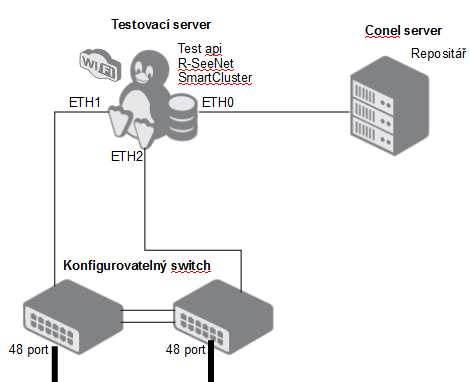
\includegraphics[width=.4\LW]{server_switch}
  \caption{Adresářová struktura testovacího systému}
  \label{fig:server_switch}
\end{figure}

\section{Struktura databáze}

\section{Popis programu}

O průběh celého testu se stará program testlab. Testlab je program psaný v jazyc C. Program po spuštění otevře systémový log pro možnost logování chyb do systémového logu. Filtrováný systémový log by měl později být zobrazován na webowém rozhraní testovacího systému. První hláškou do systémového logu je informace o spuštění programu testlab, daným uživatelem a v určený čas. Po otevření systémového logu program rozebírá parametry na příkazové řádce. Parametry jsou rozebíráný pomocí funkce getopts. Pomocí parametrů lze ovlivnit chování programu testlab !!!!!DOPLNIT PARAMETRY!!!!!!

\begin{figure}[h]
  \centering
  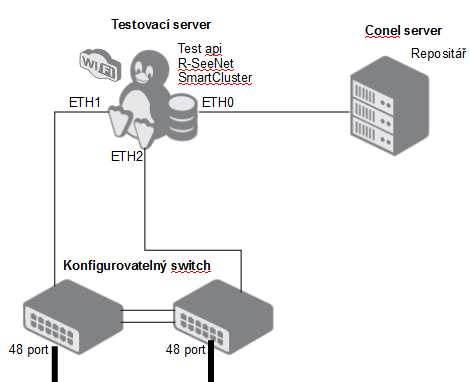
\includegraphics[width=.4\LW]{server_switch}
  \caption{Zapojení testovacího serveru a switchů}
  \label{fig:server_switch}
\end{figure}


Nyní se provádějí přípravné kroky pro samotné testování. Nejdříve je vytvořen nový release firmwaru a následně vložen do databáze. V projektovém adresáři je vytvořen nový adresář se stejným názvem jako identifikační číslo testovaného releasu.

\section{Checkout}
\section{Compile}
\section{Test router}
\section{Test tunel}
\section{Clean}
\section{Remote server}
\subsection{Telnet}
\subsection{SSH}

\endinput
